\begin{figure}[!htb]
  \centering
  \begin{subfigure}{0.08\textwidth}
    \centering
    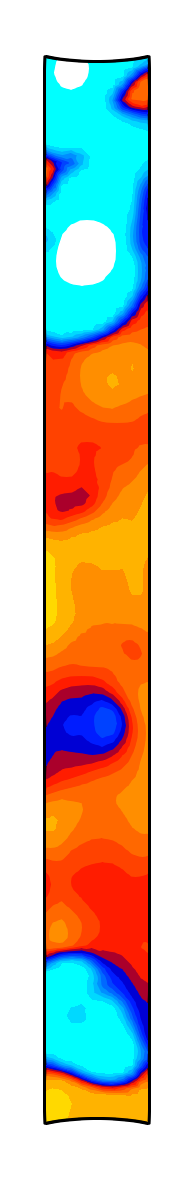
\includegraphics[width=\textwidth]{Chapter5/figures/spallation/c_1}
  \end{subfigure}
  \begin{subfigure}{0.08\textwidth}
    \centering
    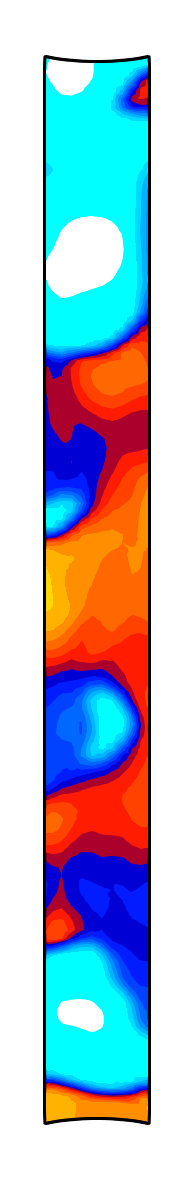
\includegraphics[width=\textwidth]{Chapter5/figures/spallation/c_2}
  \end{subfigure}
  \begin{subfigure}{0.08\textwidth}
    \centering
    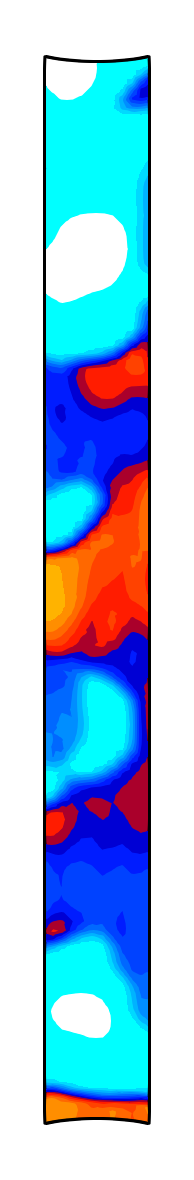
\includegraphics[width=\textwidth]{Chapter5/figures/spallation/c_3}
  \end{subfigure}
  \begin{subfigure}{0.08\textwidth}
    \centering
    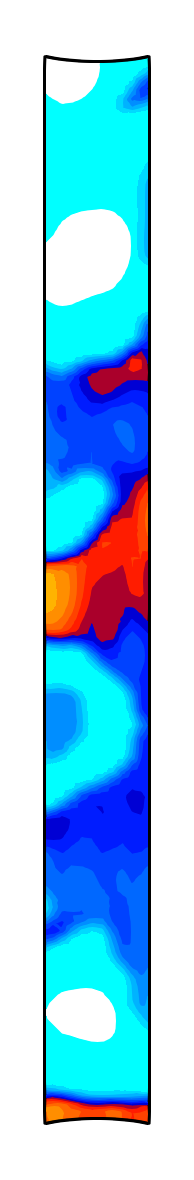
\includegraphics[width=\textwidth]{Chapter5/figures/spallation/c_4}
  \end{subfigure}
  \begin{subfigure}{0.08\textwidth}
    \centering
    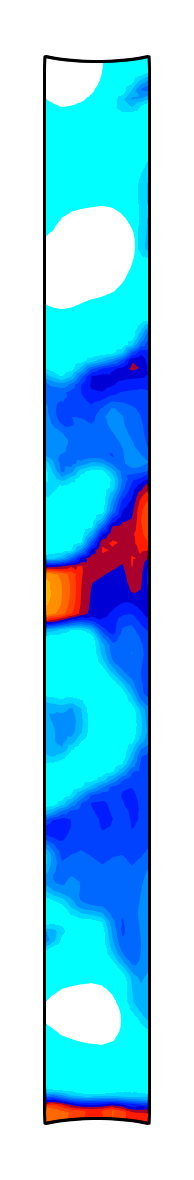
\includegraphics[width=\textwidth]{Chapter5/figures/spallation/c_5}
  \end{subfigure}
  \begin{subfigure}{0.08\textwidth}
    \centering
    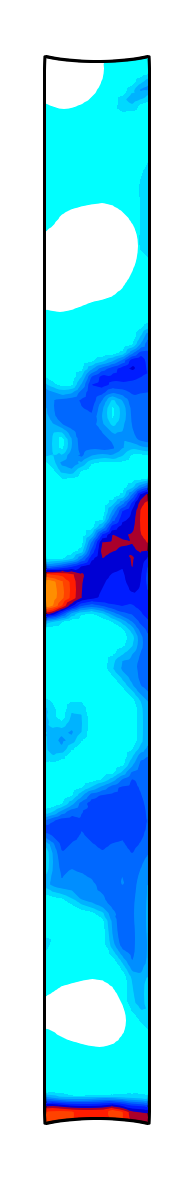
\includegraphics[width=\textwidth]{Chapter5/figures/spallation/c_6}
  \end{subfigure}
  \begin{subfigure}{0.08\textwidth}
    \centering
    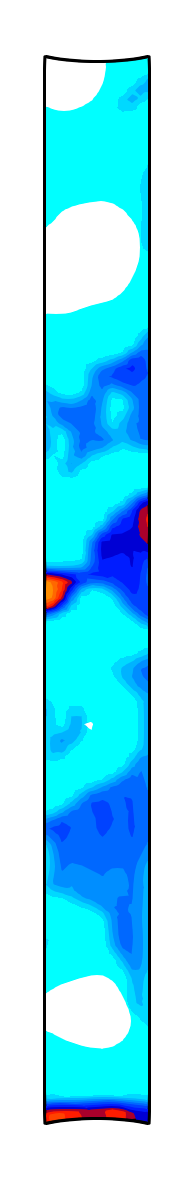
\includegraphics[width=\textwidth]{Chapter5/figures/spallation/c_7}
  \end{subfigure}
  \begin{subfigure}{0.08\textwidth}
    \centering
    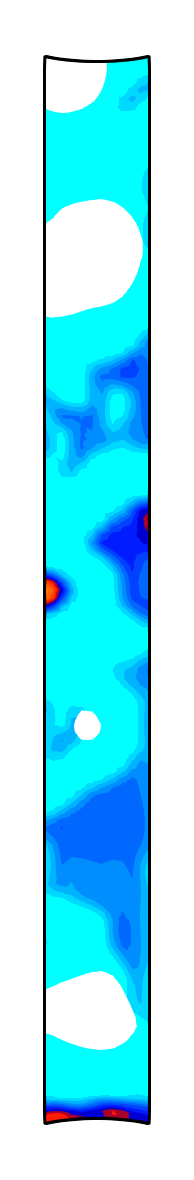
\includegraphics[width=\textwidth]{Chapter5/figures/spallation/c_8}
  \end{subfigure}
  \begin{subfigure}{0.08\textwidth}
    \centering
    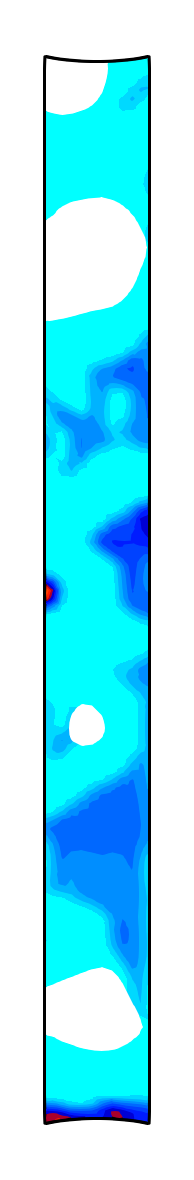
\includegraphics[width=\textwidth]{Chapter5/figures/spallation/c_9}
  \end{subfigure}
  \begin{subfigure}{0.08\textwidth}
    \centering
    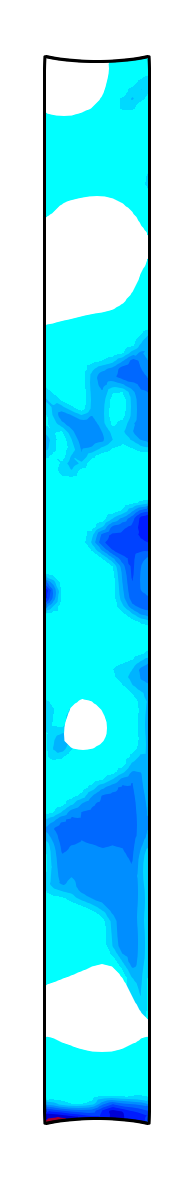
\includegraphics[width=\textwidth]{Chapter5/figures/spallation/c_10}
  \end{subfigure}
  \begin{subfigure}{0.1\textwidth}
    \centering
    \caption*{$c$}
    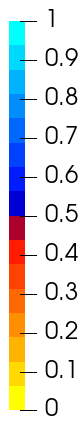
\includegraphics[width=0.8\textwidth]{Chapter5/figures/spallation/colorbar_c}
  \end{subfigure}
  \caption{The debonding indicator right after each shut-down event. The region within the contour of $d = 0.75$ is removed to visualize in-plane fracture.}
  \label{fig: Chapter5/spallation/animation_c}
\end{figure}
